\section{Задание}

Создать генератор сказок. Ввод данных в текстовые поля формы. Сгенерированную сказку вывести в другое окно.

\begin{center}
  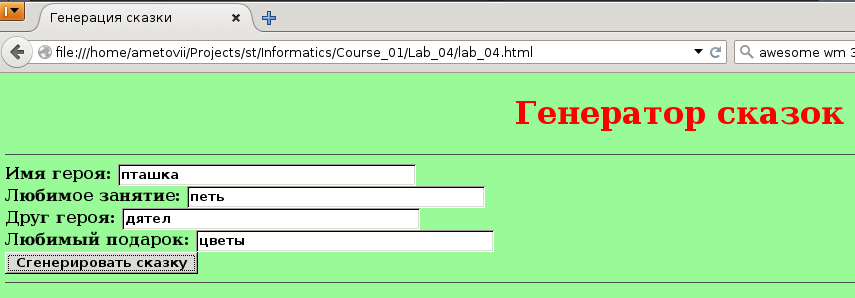
\includegraphics[width=15cm]{img/01.png}

  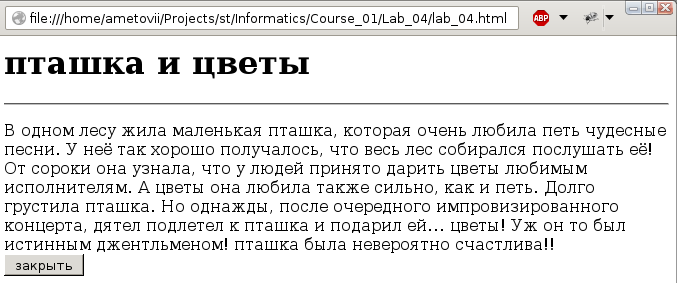
\includegraphics[width=15cm]{img/02.png}
\end{center}

Исходный код \verb|lab_04.html|:

\begin{verbatim}
<!doctype html>
<html>
  <head>
    <title>Генерация сказки</title>
    <meta charset='utf-8' />
    <style>
      h1 {color:red; text-align:center;}
      body {background-color:PaleGreen; font-weight:bold;}
      input {font-weight:bold;}
    </style>
    <script>
      function genStory()
      {
	  var heroName=document.getElementById('heroName').value;
	  var hobby=document.getElementById('hobby').value;
	  var heroFriend=document.getElementById('heroFriend').value;
	  var bestGift=document.getElementById('bestGift').value;
	  var win=window.open("", "", "width=400, height=500");
	  win.document.open();
	  var str="<h1>"+heroName+" и "+bestGift+"</h1><hr><P>";
	  win.document.write(str);
	  str='В одном лесу жила маленькая '+heroName+
	      ', которая очень любила '+hobby+
	      ' чудесные песни. У неё так хорошо '+
	      'получалось, что весь лес собирался '+
	      'послушать её! От сороки она узнала,'+
	      ' что у людей принято дарить '+bestGift+
	      ' любимым исполнителям. А '+bestGift+
	      ' она любила также сильно, как и '+hobby+
	      '. Долго грустила '+heroName+'. Но однаж'+
	      'ды, после очередного импровизированного'+
	      ' концерта, '+heroFriend+' подлетел к '+
	      heroName+' и подарил ей... '+bestGift+
	      '! Уж он то был истинным джентльменом! '+
	      heroName+' была невероятно счастлива!!<br>';
	  win.document.write(str);
	  str='<input type="button" value="закрыть"'+
	      ' onClick="window.close();">';
	  win.document.write(str);
	  win.document.close();
      }
    </script>
  </head>
  <body>
    <h1>Генератор сказок</h1>
    <hr>
    <form>
      Имя героя: <input type=text value="пташка"
			name="heroName" id='heroName' size="30"><br>
      Любимое занятие: <input type=text value="петь"
			      name="hobby" id='hobby' size="30"><br>
      Друг героя: <input type=text value="дятел"
			 name="heroFriend" id='heroFriend' size="30"><br>
      Любимый подарок: <input type=text value="цветы"
			      name="bestGift" id='bestGift' size="30"><br>
      <input type=button value="Сгенерировать сказку"
	     OnClick="genStory()">
      <hr>
    </form>
  </body>
</html>
\end{verbatim}
